\documentclass{tnreport}
%documentclass[stage2a]{tnreport} % If you are in 1nd year
%\documentclass[stage2a]{tnreport} % If you are in 2nd year
%\documentclass[confidential]{tnreport} % If you are writing confidential report
%\documentclass[english]{tnreport} % If you are writing your report in english
%\documentclass dispo pour l'appentissage: pde, pe1a, prd, pe2a, pfe

\def\reportType{Etat de l'art et description}

\def\reportTitle{Rapport Projet Pluridisciplinaire} % Titre du mémoire

\def\reportAuthor{Clement GEHIN\\ Romain NATANELIC\\ Nicolas RENARD}
% This is an example, for a report with several students as authors
%\def\reportAuthor{Jon Snow\\ Samwell Tarly}
\def\reportAuthorEmail{\email{clement.gehin@telecomnancy.eu}\\ \email{romain.natanelic@telecomnancy.eu}\\ \email{nicolas.renard@telecomnancy.eu}} % Courriel de l'élève

\def\reportAuthorAddress{} % Adresse de l'élève
\def\reportAutorCity{} % Adresse (cont.) de l'élève
\def\reportAuthorPhone{} % Téléphone de l'élève

%\def\reportIndustrialSupervisor{Eddard Stark} % Prénom Nom de l'encadrant industriel
\def\reportSupervisor{Eddard Stark} % Prénom Nom de l'encadrant industriel (en entreprise ou laboratoire)
\def\reportAcademicSupervisor{Tyrion Lannister} % Prénom Nom de l'encadrant académique

% For PIDR ?
%\def\reportSupervisor{Eddard Stark} % Prénom Nom de l'encadrant industriel
%\def\reportProjectCustomer{Projet réalisé pour l'équipe Night's Watch du laboratoire HBO}

\def\reportCompany{} % Nom de l'entreprise d'accueil
\def\reportCompanyAddress{}  % Adresse de l'entreprise
\def\reportCompanyCity{} % Adresse (cont.) de l'entreprise
\def\reportCompanyPhone{} % Téléphone de l'entreprise
\def\reportCompanyLogoPath{} % Logo de l'entreprise -- comment this definition to remove company logo

\def\place{Villers les Nancy} % Ville pour la signature pour l'engagement anti-plagiat
\def\date{\today} % Date pour la signature de l'engagement anti-plagiat

%externalisable dans un .gls
\newglossaryentry{tem}
{
	name={TEM},
	description={scanning electron microscope}
}

\begin{document}

\maketitle
\pagenumbering{roman}

\insertAntiPlagiarismAgreement{GEHIN Clement}{32010615}
\insertAntiPlagiarismAgreement{NATANELIC Romain}{31914357}
\insertAntiPlagiarismAgreement{RENARD Nicolas}{31912191}

% You may insert several agreement in case of multiple authors
%\insertAntiPlagiarismAgreement{Tarly, Samwell}{2014031142}

\cleardoublepage

\makesecondtitle

\renewcommand{\baselinestretch}{0.5}\normalsize
\tableofcontents
\renewcommand{\baselinestretch}{1.0}\normalsize
\cleardoublepage

\pagenumbering{arabic}
\setcounter{page}{1}

\section*{Etat de l'art}
\addcontentsline{toc}{chapter}{Etat de l'art}
\subsection*{L'existant}
\addcontentsline{toc}{section}{L'existant}
\begin{sloppypar}
    Avant de démarrer ce projet, il a fallu rechercher l'existant, les solutions qui étaient déjà commercialisées ou qui étaient déjà mises en place. L'objectif étant de ne pas réaliser une application déjà existante d'une part, mais aussi d'autre part de déterminer des critères pour notre application afin de connaître les éléments essentiels et les fonctionnalités que nous aimerions réaliser. C'est ce que l'on appelle l'Etat de l'Art.\\
    \\
    Pour lister les éléments existants, nous avons choisi de créer un tableau coopératif dans lequel nous allions chacun choisir un site existant et que nous devions alors analyser. Chacun de nous allait pouvoir déterminer des caractéristiques auxquelles le site répond ou non. Voici un aperçu de ce tableau : \\
    \\
    \begin{figure}[h]
        \centering
        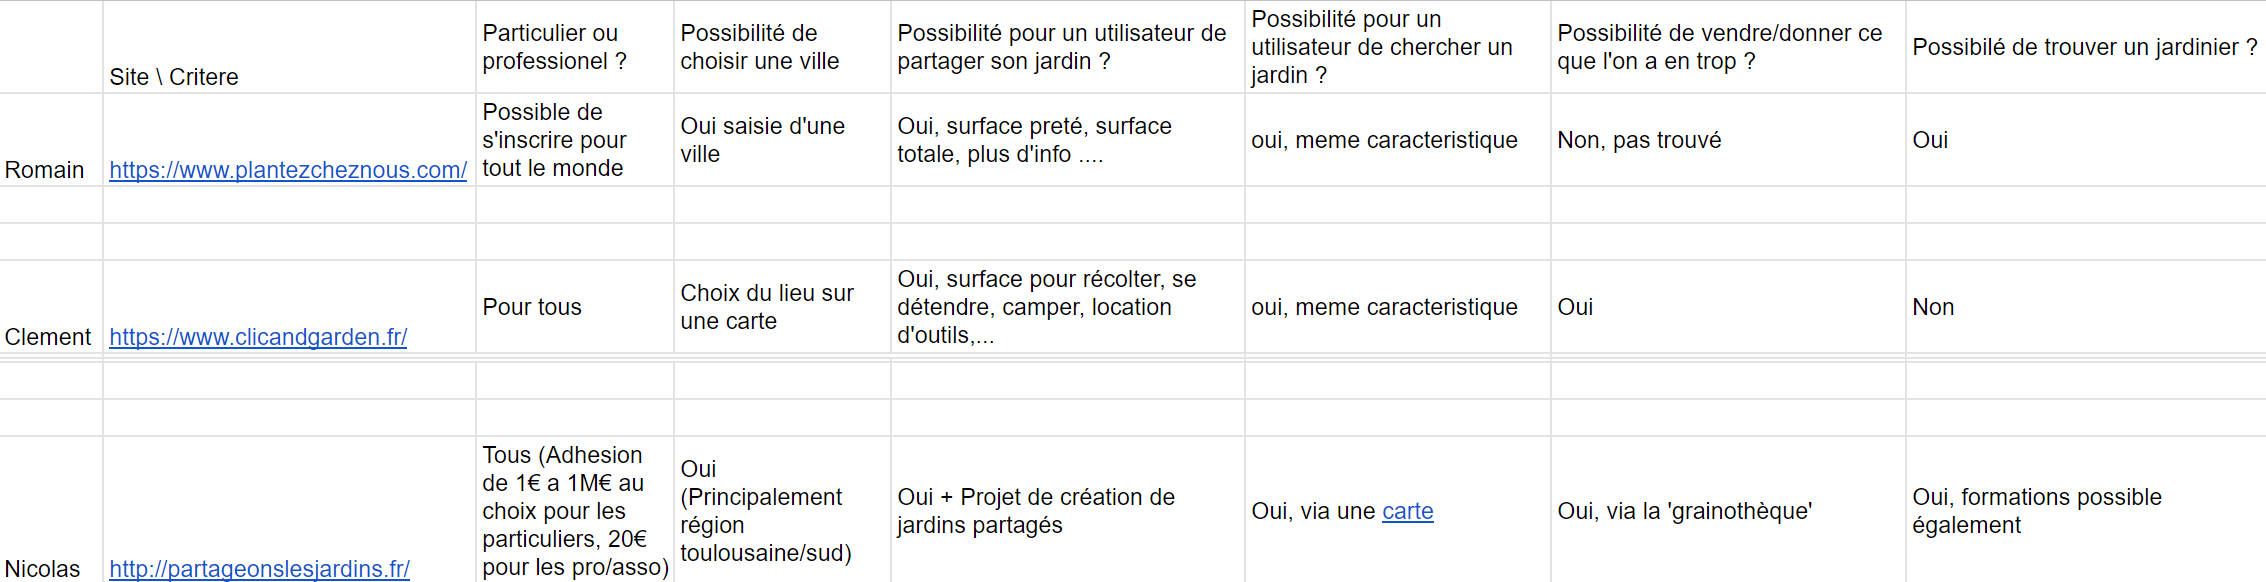
\includegraphics[scale=0.48]{Image/tableauEtatDeLArt.png}
        \caption{Recherche des critères}
        \label{fig:etat de l'Art}
    \end{figure}
    \\
    Nous avons donc déterminé les critères en colonnes, en fonction des idées que nous pouvions avoir, ou de ce que le site proposait. Cela permet de déterminer des attentes qui sont non seulement personnelles, mais reflètent par la même occasion les attentes des consommateurs, et donc de notre futur public.
\end{sloppypar}

\subsection*{Critère retenus}
\addcontentsline{toc}{section}{Critère retenus}
\begin{sloppypar}
Après avoir fait la liste des sites existant dans ce domaine, nous avons réalisé une réunion (dont le compte rendu est disponible) pour échanger sur les critères de notre futur site.\\
\\
Suite à cette réunion, nous avons retenu les critères suivants : 
\\
Nous voulons qu'elle permette aux personnes possédant un jardin, de  faire profiter aux étudiants des légumes et fruits que les foyers auraient en trop.
\\
Cela aurait deux objectifs. Tout d'abord, permettre aux étudiants, l'une des populations les plus précaires en France, de pouvoir s'alimenter en échange d'une légère main-d'oeuvre ou en tenant compagnie aux personnes âgées, par exemple, et qui nous amènerait donc vers notre deuxième objectif, qui serait de faire face à l'isolement des personnes âgées, mais également des étudiants qui se retrouvent souvent seuls dans leur logement.\\
\\
Nous souhaitons également développer, au sein de notre application, une partie qui pourrait s'apparenter à un blog, où les utilisateurs pourraient donner des conseils sur la manière de cuisiner certains aliments ou encore sur la manière de les cultiver chez soi.
\end{sloppypar}

\subsection*{Choix techniques}
\addcontentsline{toc}{section}{Choix techniques}
\begin{sloppypar}
    Pour ce qui est des choix techniques concernant le site, nous avons certaines libertés mais aussi des obligations : \\
    \begin{itemize}
        \item[\textbullet] Nous devons utiliser Python ainsi que Flask qui est un framework pour Python. Pour la persistance des données, une base de données relationnelle nous est imposée.\\
        \item[\textbullet] Pour les libertés, en commençant par la base de données, nous utiliserons une base de données MySQL qui est une base sur laquelle nous avons tous un minimum d'expérience. Nous utiliserons également SQLAlchemy qui est un ORM pour Python. Cela facilitera l'usage de la base de données à travers le site.\\
    \end{itemize}
    \\
    Un autre choix technique important est la structure du projet. Nous allons construire notre projet selon la méthode MVC avec une particularité, la version MVC-M.\\
    MVC correspond à Modele, Vue, Controller. Le Modele contient toutes les classes métiers de l'application, la Vue contient toutes les pages qui seront affichées et les Controller vont faire les liens entre la Vue et le Modele. La particularité avec la version MVC-M est que l'on ajoute un Manager, qui va contenir des méthodes qui pourront être réutilisées, pour le Modele ou pour du traitement de manière générale.\\
    Cela permet également de décomposer les différents traitements et processus. 
\end{sloppypar}

\clearpage
\section*{Gestion de projet}
\addcontentsline{toc}{chapter}{Gestion de projet}
\subsection*{Notre équipe}
\addcontentsline{toc}{section}{Notre équipe}
\begin{sloppypar}
    Ce projet est, pour nous 3, notre premier projet commun. Il est donc important d'apprendre à nous connaitre, autant dans les méthodes de travail que dans nos compétences respectives.\\
    \\
    Pour être au courant nos points forts respectifs, il est impératif de connaître les forces et faiblesses de chacun dans les différents domaines de développement. C'est pourquoi nous avons choisi de définir des référents selon 3 grandes parties :\\
    \begin{itemize}
        \item[\textbullet]Base de données : NATANELIC Romain
        \item[\textbullet]Frontend : GEHIN Clement
        \item[\textbullet]Backend : RENARD Nicolas\\
    \end{itemize}
    Avec ces différents rôles de "référents", nous allons pouvoir travailler tour à tour sur des tâches qui toucheront à chacunes de ces parties, et il est donc important pour nous de savoir vers qui se tourner dans le groupe en cas de problèmes. La personne "experte" du domaine pourra donc intervenir sur le souci, ce qui évitera de ralentir le projet, et ne bloquera pas son avancée .\\
    \\
    Cela va également nous permettre à chacun de monter en compétences car, même si nous ne sommes pas assignés à un domaine, nous allons tout de même devoir effectuer des tâches qui concernent ce dernier. De ce fait, s'améliorer pas à pas afin d'être plus performant dans les domaines qui ne sont pas nos forces.
\end{sloppypar}

\subsection*{Nos forces et faiblesses}
\addcontentsline{toc}{section}{Nos forces et faiblesses}
\begin{sloppypar}
    En ce qui concerne nos forces et nos faiblesses, nous avons choisi de nous inspirer de la matrice SWOT afin de les déterminer. La seule contrainte étant que l'extérieur n'affecte pas notre projet, outre la charge de travail déjà présente. Nous allons donc uniquement référencer les forces et faiblesses interne à notre équipe.\\
    \\
    Nos forces : \\
    \begin{itemize}
        \item [\textbullet] Nous possédons tous des compétences en informatique ce qui permet de ne pas découvrir certains domaines comme le développement par exemple.
        \item [\textbullet] Notre groupe possède des compétences dans les 3 piliers que nous avons définis, ce qui permet au projet de ne pas avoir de lacune dans un domaine particulier.
        \item [\textbullet] Nous partageons une très bonne entente entre les différents membres du groupe, ce qui facilitera la communication ainsi que l'entraide.\\
    \end{itemize}
    \\
    Nos faiblesses : \\
    \begin{itemize}
        \item [\textbullet] Nous sommes un groupe de 3 et non de 4 comme les autres groupes, ce qui signifie que la charge de travail sera plus importante et que nous devrons fournir encore plus d'efforts.
        \item [\textbullet] Du fait que nous sommes en apprentissage, nous sommes une partie du temps en entreprise et l'autre partie en cours, ou les semaines sont relativement denses, ce qui fait que nous avons moins de temps disponible que les groupes en filières initiales.
        \item [\textbullet] Nous ne possédons aucune connaissance sur les jardins partagés, ce qui pourra être handicapant par moment.
        \item [\textbullet] Enfin, aucun de nous n'a déjà travaillé avec Flask, ce sera donc une découverte pour nous et il y aura un apprentissage de ce Framework à faire.\\
    \end{itemize}
\end{sloppypar}

\subsection*{Planification}
\addcontentsline{toc}{section}{Planification}
\begin{sloppypar}
    Nous avons choisi de réaliser une planification des différentes tâches que l'on a déterminées. Cette planification est disponible \href{https://humane-wasp-582.notion.site/5f64fa977cbc4b168b634499d80aa1f3?v=48621b47058942d49c3964062fba6310}{sur cette page}. \\
    \\
    Nous avons choisi de faire notre planification sur le site Notion car il est simple d'usage et permet de faire une planification assez avancée avec différents indicateurs.
    \\
    Cette planification n'est pas un diagramme de Gantt même s'il s'en rapproche. Nous avons indiqué notre chemin critique, les prédécesseurs de certaines tâches ou encore la durée estimée d'une tâche.\\
    \\
    Cela va permettre de nous attribuer les tâches principales à effectuer, les assigner aux différents membres de l'équipe mais aussi de créer un espace de discussion pour chaque tâches afin de pouvoir séparer chaque discussion.
\end{sloppypar}

\end{document}